\documentclass[crop,tikz,border=1px]{standalone}

\usetikzlibrary{arrows,positioning,scopes,automata,calc}

\begin{document}
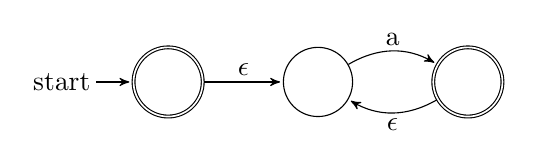
\begin{tikzpicture}[remember picture,
  ->,>=stealth',shorten >=1pt,auto,node distance=1cm,inner sep=2pt,
  mystate/.style={state,text centered}]

  \node[initial,accepting,mystate] (q0) {};
  \node[mystate] (q1) [right=of q0] {};
  \node[accepting,mystate] (q2) [right=of q1] {};

  \path (q0) edge node [above] {\(\epsilon\)} (q1)
        (q1) edge [bend left] node [above] {a} (q2)
        (q2) edge [bend left] node [below] {\(\epsilon\)} (q1);

\end{tikzpicture}
\end{document}
